\item Se a corda é submetida a uma força horizontal $P=\SI{150}{\newton}$, e a engrenagem está suportada por um pino fixo em $O$, determine a velocidade angular da engrenagem e a velocidade da cremalheira de \SI{20}{\kilogram} em \SI{4}{\second}, partindo do repouso. A massa da engrenagem é \SI{50}{\kilogram} e ela tem um raio de giração $k_{O}=\SI{125}{\milli\meter}$. Suponha
que a superfície de contato entre a cremalheira e o plano horizontal é lisa.

\import{../answers}{answer-4}

\vspace{-1.85cm}
\begin{flushright}
	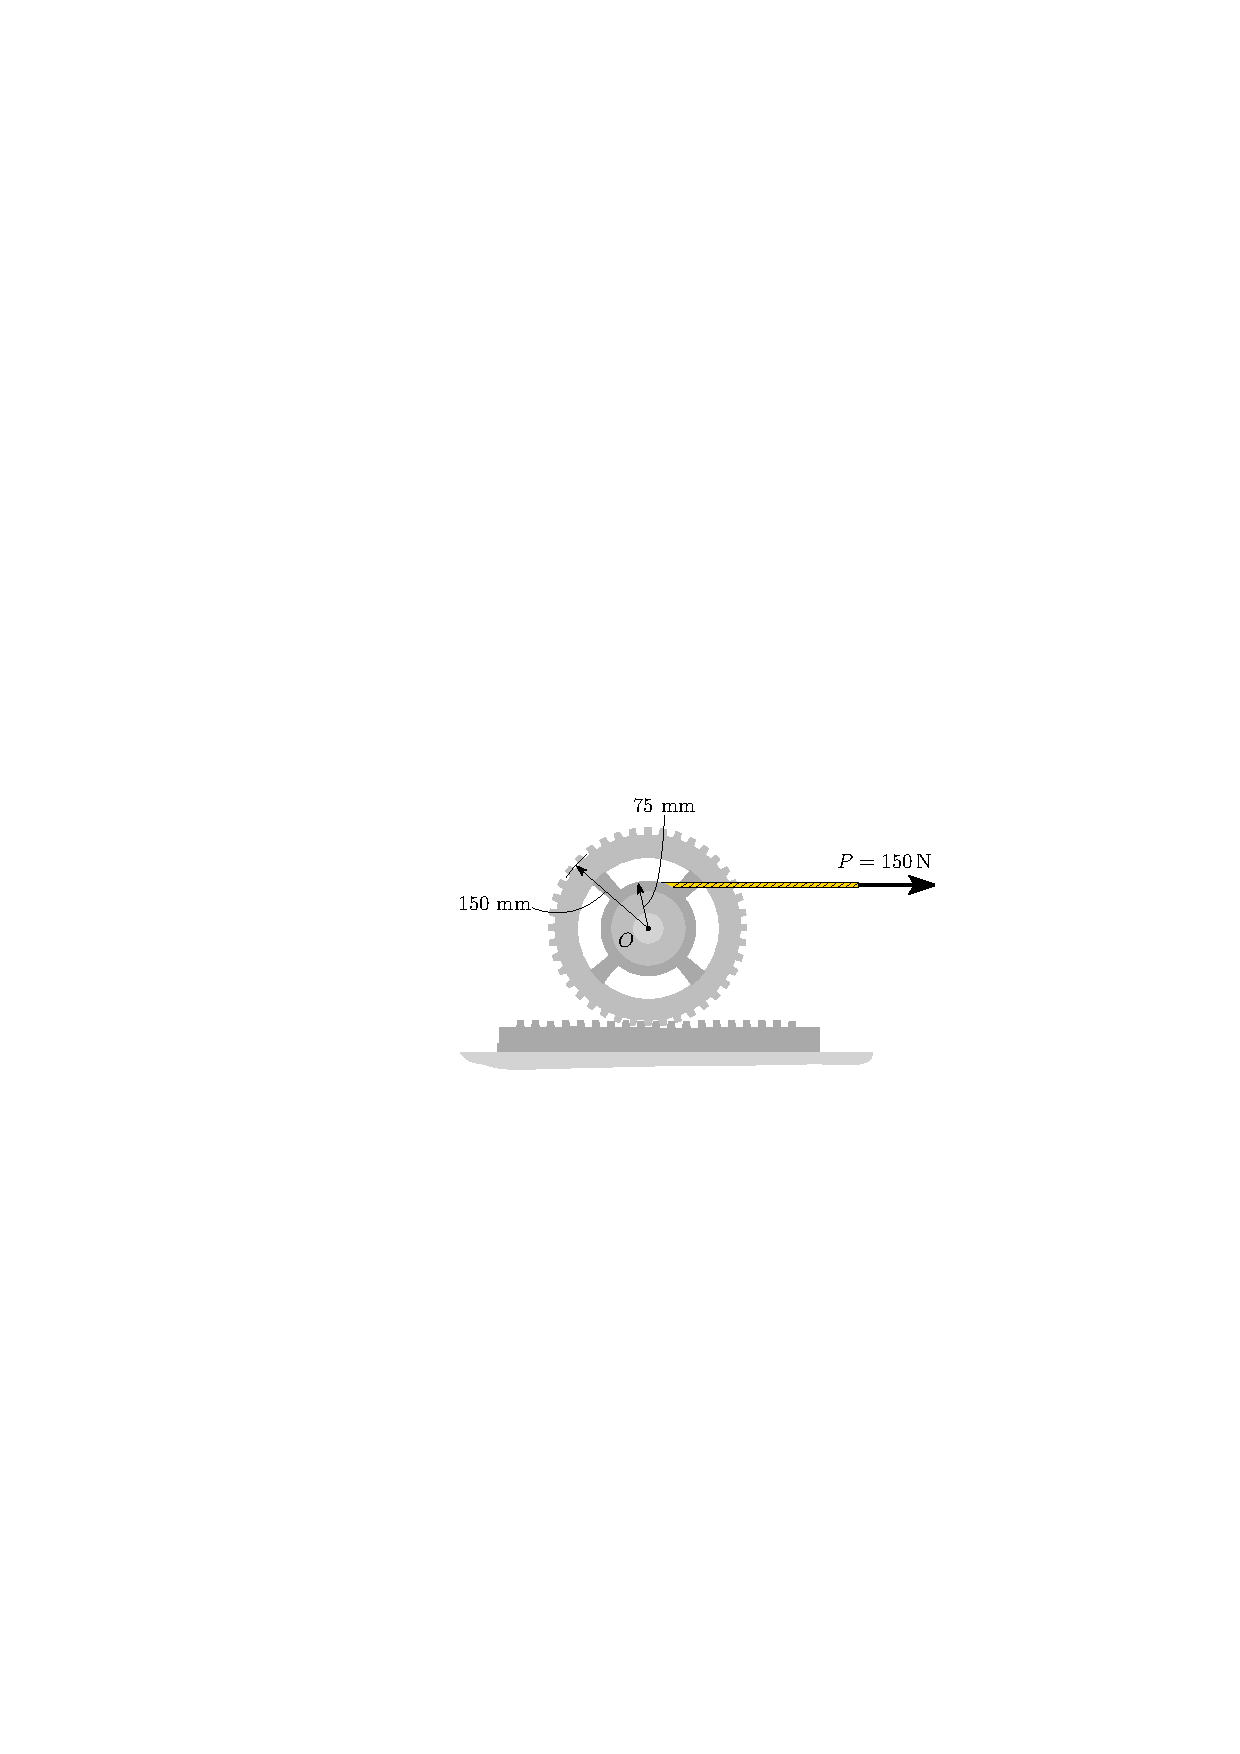
\includegraphics[scale=1.2]{../../images/draw_2}
\end{flushright}
